\documentclass[
	10pt,								% globale Schriftgröße
	parskip=half-,						% setzt Absatzabstand hoch
	paper=a4,							% Format
	english,ngerman,					% lädt Sprachpakete
	]{scrartcl}							% Dokumentenklasse

% //////////////////// Pakete laden ////////////////////
\usepackage{amsmath}			% MUSS vor fontspec geladen werden
\usepackage{mathtools}			% modifiziert amsmath
\usepackage{amssymb}			% mathematische symbole, für \ceckmarks
\usepackage{amsthm}				% für proof
\usepackage{mathrsfs}			% für \mathscr
\usepackage{latexsym}
\usepackage{marvosym}				% für Lightning

\usepackage{fontspec} 			% funktioniert nur mit den neueren Compilern z.B. XeLaTeX
\usepackage{microtype}			% für bessere Worttrennung
\usepackage[ngerman]{babel} 	% Spracheinstellung
\usepackage{lmodern}			% verändert verwendete Schriftart, damit sie weniger pixelig ist

\usepackage{verbatim}
\usepackage{listings}			% Für Quellcode

\usepackage{graphicx}
\usepackage{tabularx}			% für Tabellen mit gleicher Spaltenbreite und automatischen Umbrüchen
\usepackage{fullpage}
\usepackage{multirow}			% für multirow in tabulars
\usepackage{rotate}
\usepackage[cmyk,table]{xcolor} % um Farben zu benutzen, kann mehr als das Paket color
\usepackage[					% Verlinkungen
	colorlinks,					% farbige Schrift, statt farbiger Rahmen
	linktocpage,				% verlinkt im Abb.Verzeichnis Seitenzahl statt Bildunterschrift
	linkcolor=blue				% setzt Farbe der Links auf blau
	]{hyperref}					% nur für digitale Anwendungen, url = "http://www.example.com"
\usepackage{url}				% für Webadressen wie e-mail usw.: "\url{http://www.example.com}"

\usepackage{enumerate}			% für versch. Aufzählungezeichen wie z.B. a)
\usepackage{xspace}				% folgt ein Leerzeichen nach einem \Befehl, wird es nicht verschluckt.
\usepackage{cancel}				% für das Durchstreichen u.a. in Matheformeln mit \cancel
\usepackage{float}              % zum Forcieren der Position von figure-Umgebungen

% zum Zeichnen (u.a. von Graphen)
\usepackage{fp}
\usepackage{tikz}
\usetikzlibrary{tikzmark}			% für \tikzmark{toRemember}
\usetikzlibrary{positioning}	% verbesserte Positionierung der Knoten
\usetikzlibrary{automata}		% für Automaten (GTI)
\usetikzlibrary{arrows}
\usetikzlibrary{shapes}
\usetikzlibrary{decorations.pathmorphing}
\usetikzlibrary{decorations.pathreplacing}
\usetikzlibrary{decorations.shapes}
\usetikzlibrary{decorations.text}

% //////////////////// Syntaxhighlighting ////////////////////
\lstloadlanguages{Python, Haskell, [LaTeX]TeX, Java}
\lstset{
   basicstyle=\footnotesize\ttfamily,	% \scriptsize the size of the fonts that are used for the code
   backgroundcolor = \color{bgcolour},	% legt Farbe der Box fest
   breakatwhitespace=false,	% sets if automatic breaks should only happen at whitespace
   breaklines=true,			% sets automatic line breaking
   captionpos=t,				% sets the caption-position to bottom, t for top
   commentstyle=\color{codeblue}\ttfamily,% comment style
   frame=single,				% adds a frame around the code
   keepspaces=true,			% keeps spaces in text, useful for keeping indentation
							% of code (possibly needs columns=flexible)
   keywordstyle=\bfseries\ttfamily\color{codepurple},% keyword style
   numbers=left,				% where to put the line-numbers;
   							% possible values are (none, left, right)
   numberstyle=\tiny\color{codegreen},	% the style that is used for the line-numbers
   numbersep=5pt,			% how far the line-numbers are from the code
   stepnumber=1,				% nummeriert nur jede i-te Zeile
   showspaces=false,			% show spaces everywhere adding particular underscores;
							% it overrides 'showstringspaces'
   showstringspaces=false,	% underline spaces within strings only
   showtabs=false,			% show tabs within strings adding particular underscores
   flexiblecolumns=false,
   tabsize=1,				% the step between two line-numbers. If 1: each line will be numbered
   stringstyle=\color{orange}\ttfamily,	% string literal style
   numberblanklines=false,				% leere Zeilen werden nicht mitnummeriert
   xleftmargin=1.2em,					% Abstand zum linken Layoutrand
   xrightmargin=0.4em,					% Abstand zum rechten Layoutrand
   aboveskip=2ex, 
}

\lstdefinestyle{py}{
   language=Python,
}
\lstdefinestyle{hs}{
   language=Haskell,
}
\lstdefinestyle{tex}{
	language=[LaTeX]TeX,
	escapeinside={\%*}{*)},     % if you want to add LaTeX within your code
	texcsstyle=*\bfseries\color{blue},% hervorhebung der tex-Schlüsselwörter
	morekeywords={*,\$,\{,\},\[,\],lstinputlisting,includegraphics,
	rowcolor,columncolor,listoffigures,lstlistoflistings,
	subsection,subsubsection,textcolor,tableofcontents,colorbox,
	fcolorbox,definecolor,cellcolor,url,linktocpage,subtitle,
	subject,maketitle,usetikzlibrary,node,path,addbibresource,
	printbibliography},% if you want to add more keywords to the set
     numbers=none,
     numbersep=0pt,
     xleftmargin=0.4em,
}

\lstdefinestyle{java}{
	language=Java,
	extendedchars=true,		% lets you use non-ASCII characters;
   						% for 8-bits encodings only, does not work with UTF-8
}

\lstdefinelanguage[x64]{Assembler}     % add a "x64" dialect of Assembler
   [x86masm]{Assembler} % based on the "x86masm" dialect
   % with these extra keywords:
   {morekeywords={CDQE,CQO,CMPSQ,CMPXCHG16B,JRCXZ,LODSQ,MOVSXD, %
                  POPFQ,PUSHFQ,SCASQ,STOSQ,IRETQ,RDTSCP,SWAPGS, %
                  rax,rdx,rcx,rbx,rsi,rdi,rsp,rbp, %
                  r8,r8d,r8w,r8b,r9,r9d,r9w,r9b}
}					% for 8-bits encodings only, does not work with UTF-8

\lstdefinestyle{c}{
	language=c,
	extendedchars=true,		% for 8-bits encodings only, does not work with UTF-8
}

% //////////////////// eigene Kommandos ////////////////////
\newcommand\FU{Freie Universität Berlin\xspace}% benötigt package xspace
\newcommand\gdw{g.\,d.\,w.\xspace}
\newcommand\oBdA{o.\,B.\,d.\,A.\xspace}
\newcommand{\Eu}{\texteuro}
\newcommand\N{\mathbb{N}\xspace}
\newcommand\Q{\mathbb{Q}\xspace}
\newcommand\R{\mathbb{R}\xspace}
\newcommand\Z{\mathbb{Z}\xspace}
\newcommand\ohneNull{\ensuremath{\backslash\lbrace 0\rbrace}}% \{0}
\let\dhALT\dh	% Schreibt Befehl \dh in \dhALT um
\renewcommand\dh{d.\,h.\xspace}	%renew überschreibt command \dh
\newcommand\Bolt{\;\text{\LARGE\raisebox{-0.3em}{\Lightning}\normalsize}\xspace}% Blitz
\newcommand\zz{\ensuremath{\raisebox{+0.25ex}{Z}% zu zeigen
			\kern-0.4em\raisebox{-0.25ex}{Z}%
			\;\xspace}}
\newcommand{\from}{\ensuremath{\colon}}
\newcommand{\floor}[1]{\lfloor{#1}\rfloor}
\newcommand{\ceil}[1]{\lceil{#1}\rceil}
 \renewcommand{\L}{\ensuremath{\mathcal{L}}\xspace}
 \renewcommand{\P}{\ensuremath{\mathcal{P}}\xspace}
 \newcommand{\NL}{\ensuremath{\mathcal{N}\kern-0.2em\mathcal{L}}\xspace}
 \newcommand{\NP}{\ensuremath{\mathcal{NP}}\xspace}

% //////////////////// Mathefunktionen ////////////////////
\DeclareMathOperator{\Landau}{\mathcal{O}}
\DeclareMathOperator{\True}{True}
\DeclareMathOperator{\False}{False}

% //////////////////// eigene Theoreme ////////////////////
\newtheorem{theorem}{Satz}
\newtheorem{corollary}[theorem]{Folgerung}
\newtheorem{lemma}[theorem]{Lemma}
\newtheorem{observation}[theorem]{Beobachtung}
\newtheorem{definition}[theorem]{Definition}
\newtheorem{Literatur}[theorem]{Literatur}
% konfiguriert proof
\makeatletter
\newenvironment{Proof}[1][\proofname]{\par
  \pushQED{\qed}%
  \normalfont \topsep6\p@\@plus6\p@\relax
  \trivlist
  \item[\hskip\labelsep
%         \itshape
        \bfseries
    #1\@addpunct{.}]\ignorespaces
}{%
  \popQED\endtrivlist\@endpefalse
}
\makeatother

% //////////////////// eigene Farben ////////////////////
\let\definecolor=\xdefinecolor
\definecolor{FUgreen}{RGB}{153,204,0}
\definecolor{FUblue}{RGB}{0,51,102}

\definecolor{middlegray}{rgb}{0.5,0.5,0.5}
\definecolor{lightgray}{rgb}{0.8,0.8,0.8}
\definecolor{orange}{rgb}{0.8,0.3,0.3}
\definecolor{azur}{rgb}{0,0.7,1}
\definecolor{yac}{rgb}{0.6,0.6,0.1}
\definecolor{Pink}{rgb}{1,0,0.6}

\definecolor{bgcolour}{rgb}{0.97,0.97,0.97}
\definecolor{codegreen}{rgb}{0,0.6,0}
\definecolor{codegray}{rgb}{0.35,0.35,0.35}
\definecolor{codepurple}{rgb}{0.58,0,0.82}
\definecolor{codeblue}{rgb}{0.4,0.5,1}

% //////////////////// eigene Settings ////////////////////

\textheight = 230mm		% Höhe des Satzspiegels / Layouts
\footskip = 10ex			% Abstand zw. Fußzeile und Grundlinie letzter Textzeile
\parindent 0pt			% verhindert Einrückung der 1. Zeile eines Absatzes
\setkomafont{sectioning}{\rmfamily\bfseries}% setzt Ü-Schriften in Serifen, {disposition}
\usepackage{enumitem}
\usepackage{cite}
    \bibliographystyle{IEEEtran}
\usepackage{natbib}
\newcommand{\dozent}{Dr. Larissa Groth}
\newcommand{\veranstaltung}{IoT Network Security}
\newcommand{\semester}{SoSe23}
\newcommand{\studenten}{Zohreh Asadi, Aiman Al-Hazmi}
\begin{document}
% /////////////////////// BEGIN TITLEPAGE /////////////////////////
\begin{titlepage}
	\title{\veranstaltung}
	\subtitle{\Large Untersuchung der verschieden Schutzmechanismen in Smart Home Netzwerken, \semester}
	\author{\textbf{Autoren:} \studenten \\ \textbf{Dozentin:} \dozent}
	\date{\normalsize \today}
\end{titlepage}

\maketitle								% Erstellt das Titelblatt
\vspace*{-9cm}							% rückt Logo an den oberen Seitenrand
\makebox[\dimexpr\textwidth+1cm][r]{	%rechtsbündig und geht rechts 1cm über Layout hinaus
	
\includegraphics[width=0.4\textwidth]{src/fu_logo} % fügt FU-Logo ein
}
% /////////////////////// END TITLEPAGE /////////////////////////

\vspace{6cm}							% Abstand
\rule{\linewidth}{0.8pt}				% horizontale Linie
\tableofcontents
\newpage

\section{Einführung}

By Zohreh und Aiman:

Die Bedenken hinsichtlich der Sicherheit und des Datenschutzes von IoT-Geräten nehmen zu, da Smart Homes immer beliebter und verbreiteter werden. Es gibt Hunderttausende Studien, die Sicherheitsrisiken und Gegenmaßnahmen in Smart-Home-Umgebungen identifizieren und bewerten. Dieser Artikel bietet einen Überblick über Sicherheits- und Datenschutzprobleme in Smart-Home-Netzwerken und konzentriert sich auf die Untersuchung verschiedener Schutzmechanismen. Die Rezension basiert auf einer Auswahl mehrerer Forschungsartikel und Bücher. Ziel des Beitrags ist es, einen detaillierten Überblick über die aktuellen Forschungsergebnisse zu geben und Empfehlungen und Ansichten zur Implementierung von Sicherheitsmechanismen in einer Smart-Home-Umgebung zu geben. 

Der Artikel beginnt mit einer Einführung in verschiedene Netzwerkarchitekturen und Kommunikationsprotokolle. Das Smart-Home-Netzwerk basiert auf einem grundlegenden Schichtenmodell bestehend aus der Sensor- und Aktorschicht, der Netzwerkschicht und der Anwendungsschicht. Die Kommunikation zwischen Geräten erfolgt über verschiedene Protokolle wie Wi-Fi, Bluetooth, Zigbee, Z-Wave, MQTT und CoAP. Anschließend geht er auf die Gefahren und Risiken ein, die mit Smart-Home-Netzwerken verbunden sind, und betont die Bedeutung der Sicherheit in einer IoT-Umgebung. Darüber hinaus werden verschiedene Cyberangriffe besprochen, die häufig in IoT-Anwendungen auftreten, wie zum Beispiel: B. Channel-Angriffe, selektive Umleitungsangriffe, Sybil-Angriffe und Denial-of-Service-Angriffe (DoS). 

Im weiteren Verlauf dieses Artikels werden die wichtigsten Sicherheitsmechanismen für Smart-Home-Netzwerke erörtert, wobei der Schwerpunkt auf der IoT-Authentifizierung und der Sicherheitsarchitektur liegt. Es werden Verschlüsselungs-, Authentifizierungs- und Zugriffskontrollmechanismen untersucht, darunter Technologien wie Advanced Encryption Standard (AES), Blowfish und RSA. Die Vorteile, Einschränkungen und Leistung dieser Verschlüsselungsalgorithmen werden diskutiert. Die Authentifizierung, insbesondere mittels CoAP, spielt eine wichtige Rolle bei der Gewährleistung der Sicherheit und Integrität der Kommunikation in einem Smart-Home-Netzwerk.

Insgesamt analysiert dieser Artikel Sicherheits- und Datenschutzprobleme in Smart-Home-Netzwerken und skizziert wichtige Sicherheitsmaßnahmen. Ziel ist es, das Verständnis für Cybersicherheit im Bereich IoT zu fördern und bei der Gestaltung einer sicheren Smart-Home-Umgebung zu helfen.


\newpage
\section{Grundlagen von Smart Home Netzwerken}

\subsection{Architektur von Smart Home-Netzwerken}
By Aiman:

\paragraph{IoT Architecture}\ 
In der Literatur wurden mehrere IoT-Architekturen vorgeschlagen. Die IoT-Architektur berücksichtigt wichtige Faktoren wie Dienstqualität (QoS), Datenschutz, Zuverlässigkeit, Integrität usw. [X3]. Die allgemeine IoT-Architektur sollte aus drei Hauptschichten bestehen: der  Wahrnehmungs- oder physischen Schicht, der Netzwerkschicht und der Anwendungsschicht. In diesem Abschnitt befassen wir uns mit der grundlegenden Architektur und Serviceorientierung des IoT.

\paragraph{Basic Layred architecture}\

Das wird häufig zur Strukturierung von Komponenten und zur Interaktion mit dem System verwendet. Die mehrstufige Architektur bietet einen modularen Ansatz, der Flexibilität, Skalierbarkeit und Interoperabilität bietet.[X3] In dieser Architektur ist das IoT-System in verschiedene Schichten unterteilt, die jeweils spezifische Funktionen übernehmen. 

Normalerweise gibt es drei Klassen:
\begin{enumerate}
    \item Dier Wahrnehmungsschicht ist für das Sammeln von Daten von verschiedenen Sensoren und Geräten in der physischen Welt verantwortlich. Die kognitive Schicht wandelt physische Ereignisse in digitale Daten um, die verarbeitet und übertragen werden können[X3]. 

\item Der Netzwerkschicht sorgt für die Kommunikation zwischen Geräten/Sensoren in der Erkennungsschicht und den höheren Schichten der Architektur. Es umfasst Protokolle und Technologien wie Wi-Fi, Bluetooth, Zigbee, Mobilfunknetze und andere Konnektivitätsoptionen. Diese Schicht gewährleistet eine zuverlässige Datenübertragung und verwaltet die Kommunikation zwischen Geräten[X3].

\item Der Anwendungsschicht ist die oberste Schicht der Architektur und besteht aus verschiedenen IoT-Anwendungen und -Diensten. Diese Anwendungen nutzen verarbeitete Daten, um bestimmte Funktionen wie Überwachung, Steuerung, Automatisierung, Analyse und Entscheidungsfindung zu ermöglichen. Beispiele für IoT-Anwendungen sind Smart-Home-Systeme, industrielle Überwachungssysteme, Gesundheitsüberwachung und Umweltüberwachung[X3].
\end{enumerate}
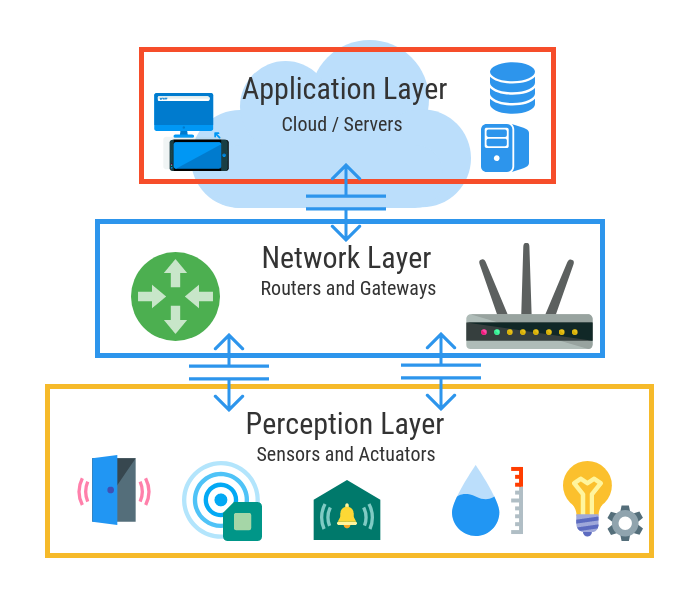
\includegraphics[scale=0.3]{resources/three-layer-iot-architecture.png}
\paragraph{Service Oriented architecture}

\paragraph{Smart Homes Architektur}\

Ein Smart Home besteht aus verschiedenen Geräten, die mit einem lokalen Netzwerk (LAN) verbunden sind. Diese Geräte kommunizieren untereinander über Kommunikationsprotokolle wie ZigBee, BLE, Wi-Fi oder andere RF-Technologien. Die Smart-Home-Architektur besteht aus einem lokalen Netzwerk, das Geräte, Sensoren und Aktoren im Haus verbindet. Ein mit dem lokalen Netzwerk verbundener Server verwaltet Geräte, protokolliert, generiert Berichte und reagiert auf Benutzerbefehle. Der Server kann auch über APIs mit Cloud-Diensten interagieren und so zusätzliche Funktionalität und Skalierbarkeit bieten. Darüber hinaus sind Smart-Home-Geräte mit dem Internet verbunden, sodass Benutzer über die Anwendung aus der Ferne auf das System zugreifen und es steuern können. Die Architektur eines IoT-basierten Smart-Home-Systems lässt sich in drei Schichten unterteilen: die Erkennungs- und Aktivierungsschicht, die Netzwerkschicht und die Anwendungsschicht.

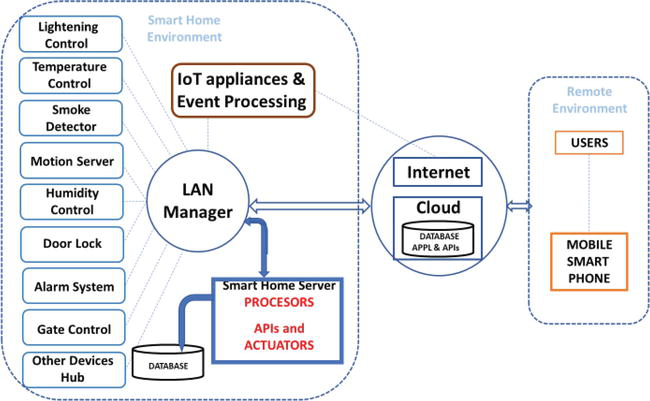
\includegraphics[scale=0.7]{resources/BuildinganIoT-basedarchitecturemodelforsmarthomes.png}

\subsection{Kommunikationsprotokolle in Smart Home Netzwerken}
By Aiman

Um in einem Smart Home effektiv kommunizieren zu können, müssen Geräte und Sensoren miteinander verbunden sein. Diese Verbindung basiert auf Kommunikationsprotokollen, die definieren, wie Informationen zwischen diesen Geräten ausgetauscht werden. Diese Protokolle werden von verschiedenen Organisationen erstellt, um eine reibungslose und standardisierte Kommunikation in Smart-Home-Umgebungen sicherzustellen.


Die Wahl des Kommunikationsprotokolls für ein Smart-Home-System hängt von vielen Faktoren ab, unter anderem Verteilungsumgebung, Netzwerkgröße, Reichweite, Datenrate, Stromverbrauch und Netzwerkkonfiguration. Kommunikationsprotokolle können in drei Hauptgruppen unterteilt werden: kabelgebunden, drahtlos und hybrid [X1]. Hier finden Sie kurze Erläuterungen zu häufig genannten Technologien für Smart-Home-Anwendungen:
\begin{enumerate}
    \item ZigBee 
    \item Bluetooth
    \item WiFi 
      \item 6LoWPAN (IPv6 over Low-Power Wireless Personal Area Networks)
          \item TLS (Transport Layer Security)
    \item Message Queuing Telemetry Transport (MQTT)
    \item Constrained Application Protocol (CoAP) 
    \item WebSocket

\end{enumerate}
\newpage
\subsection{Bedrohungen und Risiken für Smart Home-Netzwerke}

By Zohreh:

Die Gewährleistung der Sicherheit in IoT-Umgebungen ist zu einer großen Herausforderung und einem wichtigen Barriers für den Fortschritt der Smart-Home-Automatisierung geworden \cite{10.1145/1978942.1979249} .Diese Anerkennung unterstreicht ihre Komplexität und Bedeutung.
Je mehr Smart-Home- und IoT-Geräte entwickelt werden, desto schneller nehmen die mit deren Nutzung verbundenen Gefahren, Bedrohungen und Risiken zu. Hier überprüfen wir zwei verschiedene Studien. In \cite{8344666} verwenden sie eine Methode namens 'Taxonomy'; welche ist ein System zur Inhaltsverwaltung, das Informationen basierend auf als Metadaten gespeicherten Begriffen gruppiert, und durch die Analyse der vorhandenen Literatur zu Smart Homes wurde eine Reihe von Bedrohungen identifiziert, die speziell für den Bereich Smart Home gelten. Basierend auf dieser Untersuchung gibt es 28 verschiedene Arten von Threads, die in drei verschiedene Gruppen eingeteilt werden können, nämlich "Unintentional", "Malfunction" und "Intentional Threads".

\paragraph{Threads}
\

\boldsymbol{Intentional Threads:} 
Vorsätzlicher Missbrauch birgt Sicherheitsrisiken für Smart-Home-Geräte durch Aktivitäten wie Identitätsbetrug, Denial-of-Service-Angriffe und Datenmanipulation. Diese Aktionen können verschiedene zerstörerische Auswirkungen haben, darunter unbefugte Änderungen an Richtlinien, Identitätsdiebstahl und die Ausnutzung von Smart-Home-Diensten.

\boldsymbol{Malfunction Threads:} 
Ausfälle im Internet oder Hardware- oder Softwarefehler, die zu internen Störungen und Kommunikationskanalausfällen führen können, sind die häufigsten Beispiele für Störungsthreads und -risiken in Smart Homes. Ein weiteres Beispiel sind Schäden durch Geräte oder Sensoren Dritter, die zu Fehlfunktionen des Geräts führen, die einen Austausch und einen vorübergehenden Funktionsverlust erfordern. Darüber hinaus beeinträchtigt die Installation nicht vertrauenswürdiger Hardware von Drittanbietern die Gerätesicherheit.

\boldsymbol{Unintentional Threads:} 
Zu den unbeabsichtigten Threads gehören der Erhalt von Informationen aus unbekannten Quellen oder zufällige Änderungen von Daten oder Richtlinien. Dies geschieht normalerweise, wenn die Sicherheitsrichtlinien des Geräts nicht richtig eingestellt sind oder die Installation schwach ist.

In einer weiteren Studie \cite{JACOBSSON2016719} wurde die Risikoexposition von SHAS (sichere Hashing-Algorithmen) mithilfe der Methode der Information Security Risk Analysis (ISRA) untersucht.
Laut dieser Studie ist die Risikoanalyse im Internet der Dinge das größte Sperre für die Weiterentwicklung dieser Technologie. Der Zweck der Studie dieser Gruppe besteht darin, die Risiken zu verstehen, die mit der Nutzung und dem Missbrauch von Informationen in Smart Homes und Gebäuden verbunden sind, was für die Gewährleistung der Sicherheit in IoT-Umgebungen sehr wichtig ist. Von den 32 von dieser Gruppe untersuchten Risiken wurden 9 Fälle als geringes Risiko und 4 Fälle als hohes Risiko eingestuft. Hochrisikofaktoren hängen entweder mit dem menschlichen Faktor oder mit den Softwarekomponenten des Systems zusammen. 
Wenn wir die Risiken in Bezug auf Software oder Hardware kategorisieren, hängt das wahrscheinlichste Risiko in der Liste der softwarebezogenen Risiken mit einer unzureichenden Reaktionsfähigkeit des internen Gateways zusammen. Beispielsweise werden Systemereignisse nicht aufgezeichnet, was die Situation erschweren kann, später nachvollziehen. Der höchste Risikowert steht im Zusammenhang mit unbefugten Änderungen an Systemfunktionen in mobilen Anwendungen. Beispielsweise können Endbenutzer ohne entsprechende Anmeldeinformationen auf Systemressourcen zugreifen.
In der Kategorie der hardwarebezogenen Risiken sind die schwerwiegendsten Folgen hingegen mit unbefugten Änderungen bzw. Manipulationen an physischen Sensoren oder internen Gateways verbunden. Die höchsten Risikowerte beziehen sich auf unbefugte Änderungen/Manipulationen des internen Ports, beispielsweise das Zurücksetzen des Systems zur Wiederherstellung des Standardkennworts.

\paragraph{Kurzer Überblick über verschiedene Cyber-attacks}\

Einige der häufig vorkommenden Cyberangriffe auf IoT-Anwendungen:

\boldsymbol{Sinkhole-Angriff:}
Ein Sinkhole-Angriff ist eine Art Angriff auf Netzwerkebene, der auftritt, wenn Daten während der Übertragung weitergeleitet werden. Bei diesem Angriff werden alle durch das Netzwerk fließenden Daten an einen kompromittierten Knoten im Netzwerk umgeleitet \cite{7001385} .Dieser Angriff reduziert den Datenverkehr und täuscht den Absender und das Netzwerk vor, dass das Paket sein eigentliches Ziel erreicht hat. Bei diesem Angriff handelt es sich um einen aktiven Angriff, der durch die Generierung von Datenverkehr und die Unterbrechung von Routing-Pfaden zu einem Denial-of-Service-Angriff (DoS) führen kann \cite{stephen2017intrusion} .

\boldsymbol{Selektiver Weiterleitungsangriff:}
Bei diesem Angriff werden ein oder mehrere Knoten im Netzwerk von den Hackers einnimmt. Wenn einer der Knoten ein Paket als selektiven Weiterleitungsangriff verwirft, helfen andere dabei, den Angriff zu verschleiern. Dies führt zu Paketverlusten aufgrund von Interferenzen und ist schwer zu erkennen. Dieser Angriff kann dazu führen, dass unvollständige Informationen übertragen werden und deren Integrität beeinträchtigt wird. In manchen Anwendungen können unvollständige Informationen sogar gefährlicher sein als keine Informationen \cite{s16010118} .

\boldsymbol{Sybil-Angriff:}
Es ist ein weiterer Angriff auf Netzwerkebene, bei dem Angreifer Knoten manipulieren und mehrere Identitäten für einen einzelnen Knoten erstellen. Diese Art von Angriff gefährdet das gesamte System und kann zu Redundanz und falschen Informationen führen \cite{pawar2016sybil} .In IoT-Netzwerken werden Sensoren in Objekte eingebettet, die Sensorik und Kommunikation integrieren. Bei diesem Angriff wird eine gefälschte Identität generiert. Diese gefälschten Identitäten können falsche Berichte generieren, den Spam-Verkehr erhöhen und die Privatsphäre durch Malware und Phishing gefährden \cite{alqassem2014privacy} .

\boldsymbol{DoS-Angriff:}
Ein DoS-Angriff kann sowohl auf der Netzwerkebene als auch auf der Anwendungsebene erfolgen. Bei diesem Angriff überschwemmt der Angreifer das Netzwerk mit nutzlosem Datenverkehr (mehrere gleichzeitige Angriffe auf denselben Server) mit dem Ziel, Netzwerkressourcen zu belasten. Dieser Angriff macht das Netzwerk für legitime Benutzer unzugänglich \cite{kozlov2012security} .Auf der Anwendungsebene ist der Angriff sogar noch ausgefeilter, da er die Netzwerkverteidigung umgeht und vertrauliche Informationen unter der Kontrolle des Angreifers stiehlt. Dieser Angriff kann auch dazu führen, dass das gesamte Netzwerk heruntergefahren wird und nicht mehr verfügbar ist\cite{pawar2016sybil}.
\newpage

\subsection{Wichtige Schutzmechanismen zur Sicherung von Smart Home-Netzwerken} 
Um die Sicherheit eines mit dem Internet verbundenen Smart-Home-Systems zu gewährleisten, ist es wichtig, sieben Schlüsselkonzepte der Computersicherheit zu berücksichtigen und anzugehen \cite{khatoun2022cybersecurity} und [X10]:
 \begin{enumerate}
     \item Authentifizierung
\item Autorisierung
\item Vertraulichkeit
\item Integrität der Daten/Nachrichten
\item Accountability
\item Verfügbarkeit
\item Non-repudiation
 \end{enumerate}


Verschiedene Arten von Angriffen können die Sicherheit physischer Objekte oder die Sicherheit kognitiver Daten gefährden. Zum Schutz der Wahrnehmungsebene (perception layer)  sollten verschiedene Sicherheitsmethoden eingesetzt werden, darunter B. Authentifizierungs- und Zugriffskontrollverfahren, Datenintegritäts- und Sicherheitsverfahren sowie Schlüsselverwaltungssysteme [X5].

 Die Netzwerkschicht leidet unter mehreren Sicherheitsproblemen und verschiedenen Arten von Angriffen, wie z. Man-in-the-Middle-Angriffe, Listening-Angriffe, DoS-Angriffe, Replay-Angriffe, Authentifizierungsprobleme, Datenintegrität und Datenschutz, Routing-Sicherheitsprobleme und Datenschutzrisiken [X5]\cite{khatoun2022cybersecurity}


\paragraph{IoT-Sicherheitsarchitekturen}
\

IoT-Sicherheitsarchitekturen
Die IoT-Sicherheitsforschung hat zur Entwicklung verschiedener Architekturen geführt, darunter Cloud Computing (CoT), Fog Computing, Edge Computing und Gateway-Architektur. Für die Kommunikation mit IoT-Geräten werden üblicherweise Middleware-Systeme verwendet. Diese Architekturen zielen darauf ab, die Sicherheit zu verbessern und Lösungen für komplexe Verarbeitung, echtzeitnahe Reaktionen und zentralisierte Koordinationbereitzustellen. Die Gateway-Architektur bietet Proxy-Unterstützung auch dann, wenn keine Verbindung besteht.\cite{khatoun2022cybersecurity}

Hier ist eine verkürzte Liste einiger sicherer IoT-Architekturen \cite{khatoun2022cybersecurity}:

 \begin{enumerate}
     \item SH-BlockCC: Dies ist eine sichere IoT-Smart-Home-Architektur, die auf Blockchain- und Cloud-Computing-Technologie basiert. Die Blockchain-Technologie kann als wichtiger Sicherheitsmechanismus zum Schutz von Smart-Home-Netzwerken eingesetzt werden. Blockchain ist eine dezentrale und verteilte Datenbank, die Transparenz, Integrität und Sicherheit bieten kann [X13]. Das Modell verwendet die MCA-Methode (Multivariate Correlation Analysis), um den Netzwerkverkehr zu analysieren und die Korrelation zwischen Verkehrsmerkmalen zu bestimmen

    \item Smart-Home-Automatisierung mit WSN(2019): verwendet den Triangle Based Security Algorithm (TBSA), um eine energieeffiziente Datenverschlüsselung zu gewährleisten und so ein sicheres IoT-basiertes Smart-Home-Automatisierungssystem zu schaffen.

    \item IAGW(2016): Integrierte Gateway-Architektur mit Standardschnittstellen für Smart-Home-Umgebungen, inklusive Sicherheitsmodul zur Authentifizierung, Autorisierung und Verschlüsselung.

    \item IoT Cloud on CoAP(2014): Cloudbasierte IoT-Architektur basierend auf CoAP und unter Verwendung von DTLS für die Sicherheit.

    \item FIWARE (2011): ist eine IoT-Middleware mit einem Framework, das eine Vielzahl von Plugins unterstützt. Die Sicherheit wird durch Plugins für die Identitätsverwaltung, die Autorisierungspolitik und die Punkte zur Durchsetzung von Richtlinien implementiert.
 \end{enumerate}
Die folgende Tabelle fasst die Sicherheitsarchitekturen und die Sicherheitsziele zusammen, die sie jeweils zu schützen versprechen \cite{khatoun2022cybersecurity}.

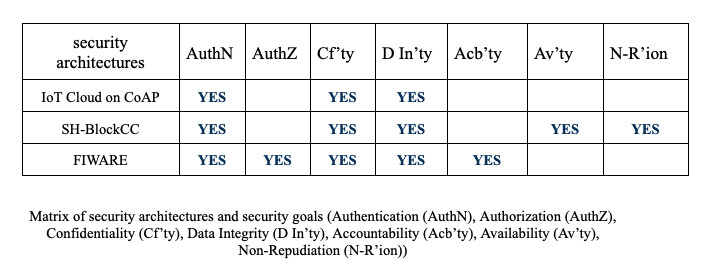
\includegraphics[scale=0.5]{resources/vergleich.png}

\paragraph{Verschlüsselung, Authentifizierung und Zugriffskontrolle}
\

Bei der Authentifizierung wird die Identität einer Person oder eines Geräts überprüft, um sicherzustellen, dass es sich um das handelt, was es vorgibt zu sein. Dieser Sicherheitsmechanismus dient dazu, unbefugten Zugriff auf das System, Daten oder Ressourcen zu verhindern. Dies werden wir genauer  später in diesem Artikel betrachten.



\paragraph{Intrusion-Detection-Systeme (IDS)}
\
Intrusion-Detection-Systeme (IDS) sind für die Netzwerk- und Datensicherheit von entscheidender Bedeutung. Sie erkennen und verhindern unbefugten Zugriff, und ein zentralisierter IDS-Ansatz kann den Einsatz bei begrenzter Stromversorgung vereinfachen. IDS arbeitet in drei Phasen: Überwachung, Analyse und Erkennung. Es verwendet Sensoren, um das Netzwerk oder den Host zu beobachten, Merkmale zu extrahieren und Muster während der Analyse zu identifizieren, und konzentriert sich bei der Erkennung auf die Identifizierung von Anomalien oder Eindringlingen. IDS entwickeln sich im Laufe der Zeit weiter und für verschiedene Systeme wurden unterschiedliche Methoden und Techniken vorgeschlagen. Durch die effiziente Verwaltung von Informationen, Diensten und Netzwerkverkehr verbessert IDS die Netzwerksicherheit, den Datenschutz und die Integrität (X10, X11).

\paragraph{Aktualisierte Firmware und Sicherheitspatches}

\newpage
\section{Verschlüsselung, Authentifizierung und Zugriffskontrolle in Smart Home-Netzwerken}
\subsection{Verschlüsselungstechnologien}

By Zohreh:

Verschlüsselungstechnologien spielen eine entscheidende Rolle bei der Sicherung von sensiblen Informationen und der Gewährleistung der Privatsphäre. 
Für die Kryptographie wurden verschiedene Ziele aufgeführt, nämlich: Vertraulichkeit, Authentifizierung, Integrität, Bestreitbarkeit und Zugangskontrolle. 

Verschlüsselungsalgorithmen können in zwei große Kategorien eingeteilt werden: Verschlüsselung mit symmetrischem Schlüssel (z. B. AES, Blowfish) und Verschlüsselung mit asymmetrischem Schlüssel (z. B. RSA).\cite{thambiraja2012survey} .
Symmetrische Verschlüsselung, auch als Geheimschlüsselverschlüsselung bekannt, ist eine grundlegende kryptografische Technik zur Sicherung sensibler Informationen. Dabei wird ein einziger geheimer Schlüssel für sowohl den Verschlüsselungs- als auch den Entschlüsselungsprozess verwendet.
Auf der anderen Seite verwendet die asymmetrische Verschlüsselung, auch bekannt als Public-Key-Verschlüsselung, ein Schlüsselpaar: einen öffentlichen Schlüssel zum Verschlüsseln von Daten und einen privaten Schlüssel zum Entschlüsseln.

Im Folgenden besprechen wir zwei symmetrische Verschlüsselungsalgorithmen, nämlich AES (Advanced Encryption Standard) und Blowfish, sowie einen asymmetrischen Verschlüsselungsalgorithmus RSA.


\subsubsection{AES:}

AES (Advanced Encryption Standard) ist ein symmetrischer Verschlüsselungsalgorithmus, der mit Datenblöcken arbeitet. Es verwendet schlüsselbasierte Ersetzungs- und Permutationsoperationen, um Vertraulichkeit und Datenintegrität sicherzustellen. AES umfasst eine Schlüsselerweiterung zur Generierung von Rundenschlüsseln und durchläuft mehrere Runden von Substitutions-, Shift-, Shuffle- und XOR-Operationen. Der Verschlüsselungsprozess wandelt Klartext in Chiffretext um, während die Entschlüsselung die Schritte umkehrt, um den ursprünglichen Klartext abzurufen.\cite{abdullah2017advanced}
The AES design is based on a substitution-permutation network 
(SPN) and does not use the Data Encryption Standard (DES) Feistel network\cite{raghav2016securing}.
Einerseits weist AES eine schlechte Leistung auf, da es mehr Rechenleistung benötigt und bei großen Datenblöcken mehr Ressourcen verbraucht. Andererseits ist es für kleine Pakete sogar besser als viele Algorithmen, einschließlich RC4, außerdem hat AES keine Wurmlöcher.\cite{abdullah2017advanced}
AES verfügt über eine schnelle Ver- und Entschlüsselung und verfügt über eine Schlüsselgröße von 128, 192 und 256 Bit. Seine Geschwindigkeit hängt vom Schlüssel ab, es ist aber sicher und funktioniert besser als viele Algorithmen, einschließlich DES und Triple-DES, und es ist sowohl in der Hardware als auch in der Software schnell\cite{devi2015review}, \cite{abdullah2017advanced}.

\subsubsection{BLOWFISH:}

Die Leistung des BLOWFISH-Algorithmus für unterschiedliche Paketgrößen mit und ohne Datentransformation ist besser als bei anderen Algorithmen und hat keine Wurmlöcher, aber er ist zeitaufwändig und verbraucht letztendlich mehr Strom\cite{thambiraja2012survey}.
Die Ver- und Entschlüsselung im BLOWFISH-Algorithmus erfolgt schnell und die Schlüsselgröße liegt zwischen 32 und 448 Bit. Die Geschwindigkeit dieses Algorithmus hängt nicht vom Schlüssel ab. Es wird angenommen, dass es gesichert ist, aber es gibt weniger Versuche zur Kryptoanalyse. Dieser Algorithmus wurde nur für Software entwickelt\cite{devi2015review}, \cite{thambiraja2012survey}.

Um die Daten mit BLOWFISH-Algorithmus zu verschlüsseln, sind folgende Schritte erforderlich:

1. Speichern Sie die Schlüssel in einem Array; k1,k2,...kn und 1<=n<=14
und die Länge jedes Blocks beträgt 32 Bit.\begin{align*}
32*14=448 \end{align*}
2. Initialisieren Sie das Array mit der Nummer p; 1<=p<=18, die Länge jedes Wortes beträgt 32 Bit.

3. Substitutions-Boxen initialisieren, jede darf maximal 255 Bit lang sein\begin{align*}
    2^8 -1 = 255 \end{align*}.
4. Initialisieren Sie jedes P-Array und S-Bixes mit Hexadezimalzahlen

5. Ausführen von XOR-Operationen zwischen k- und p-Arrays:\begin{align*} p1 = p1 XOR k1, ..., p14 = p14 XOR k14 \end{align*} \begin{align*} p15 = p15 XOR k1 , ... , p18 = p18 XOR k4.\end{align*}
6. Nehmen Sie 64-Bit-Klartexte und initialisieren Sie sie mit Null (000000).

Subkey wird generiert.
Create figure for this algo

\subsubsection{RSA:}

RSA ist ein Asymmetric-Algorithm, dasa auf Verschlüsselung mit öffentlichen Schlüsseln und digitalen Signaturen basiert hat. Bei RSA sind Verschlüsselungsschlüssel öffentlich verfügbar, während Entschlüsselungsschlüssel privat bleiben. Dadurch kann jeder eine Nachricht mit dem öffentlichen Verschlüsselungsschlüssel des Empfängers verschlüsseln, aber nur der beabsichtigte Empfänger kann sie mit dem entsprechenden privaten Entschlüsselungsschlüssel entschlüsseln. Seine Sicherheit basiert auf der Schwierigkeit von folgenden Zahlen:

„p“ und „q“: Dabei handelt es sich um unterschiedliche Primzahlen, die zufällig ausgewählt werden. Die Sicherheit von RSA beruht auf der Schwierigkeit, das Produkt dieser beiden Primzahlen zu faktorisieren. Diese Primzahlen werden geheim gehalten und zur Generierung des privaten Schlüssels verwendet.

„n“: Dies ist das Produkt der beiden Primzahlen „p“ und „q“ (n = p*q). Es ist Teil sowohl des öffentlichen als auch des privaten Schlüssels. Der Wert von „n“ ist öffentlich und kann jedem bekannt sein.
Weitere in RSA verwendete Variablen sind:

„e“: Dies ist der öffentliche Exponent, der normalerweise eine kleine Primzahl ist. Es ist Teil des öffentlichen Schlüssels und wird so gewählt, dass es eine Primzahl zum Wert von (p-1)*(q-1) ist, wodurch sichergestellt wird, dass es eine modulare Umkehrung gibt.

„d“: Dies ist der private Exponent, der aus den Primfaktoren und dem öffentlichen Exponenten abgeleitet wird. Es wird geheim gehalten und zur Entschlüsselung verwendet. Der private Exponent wird mithilfe der modularen Arithmetik und des erweiterten euklidischen Algorithmus berechnet.

Die digitale Signatur ermöglicht die Authentifizierung und Nichtabstreitbarkeit von Nachrichten. Um die Authentizität einer gesendeten Nachricht zu überprüfen, verwendet der Empfänger den Entschlüsselungsschlüssel des Absenders, um die Signatur zu entschlüsseln, die durch Verschlüsselung des Nachrichten-Hashs mit dem privaten Schlüssel des Absenders erstellt wird. Der resultierende Hash wird dann mit dem neu berechneten Hash der empfangenen Nachricht unter Verwendung des öffentlichen Verschlüsselungsschlüssels des Absenders verglichen. Wenn die beiden Hashes übereinstimmen, bestätigt dies, dass die Nachricht nicht manipuliert wurde und vom angeblichen Absender stammt.

Die Stärke der RSA-Sicherheit zeigt sich darin, dass es keine erfolgreichen Versuche gibt, sie zu knacken. Allerdings ist dieser Algorithmus im Vergleich zu symmetrischer Verschlüsselung rechenintensiv. Daher wird RSA häufig in Verbindung mit schnelleren symmetrischen Algorithmen verwendet. Darüber hinaus schaffen Timing-Angriffe und Herausforderungen im Zusammenhang mit der Schlüsselverteilung potenzielle Schwachstellen, die Gegenmaßnahmen wie spezielle Hardware- und Softwareimplementierungen erfordern. \cite{milanov2009rsa}


\subsection{Authentifizierung}

By Aiman:

In einer Welt, in der alles miteinander verbunden ist, ist die Authentifizierung der erste Schritt, um unsere Daten zu schützen. Die Authentifizierung ist ein allgemeines Sicherheitsproblem, das sich darauf auswirkt, wie wir Anwendungen wahrnehmen, verbinden und nutzen. Für das Internet der Dinge (IoT), zu dem auch Geräte mit begrenzten Ressourcen und die Cloud gehören, wurden verschiedene Arten der Authentifizierung entwickelt. Es ist wichtig zu wissen, dass sich die Authentifizierung im Laufe der Zeit kaum verändert hat, auch wenn ein einfaches Passwort in der heutigen technologiegesteuerten Welt nicht mehr ausreicht, um die Validierung des Benutzers sicherzustellen.

Es gibt mehrere Authentifizierungs- und Autorisierungsmethoden für smarte Geräte. Diese Methoden beruhen auf verschiedenen Faktoren, die sich in drei Kategorien einteilen lassen \cite{khatoun2022cybersecurity}: 1. etwas, das eine Person weiß (z. B. ein Passwort oder ein Geheimcode). 
2. etwas, das eine Person ist (z. B. ein Fingerabdruck oder ein retina pattern). 
3. etwas, das eine Person besitzt (z. B. eine Chipkarte oder ein digitaler Schlüssel).
Diese Faktoren werden verwendet, um die Identität von Personen oder Systemen in Authentifizierungs- und Autorisierungsverfahren für smarte Geräte festzustellen.


Es lassen sich zwei grundlegende Arten von Authentifizierungsmechanismen unterscheiden: Intra-Domain (Authentifizierung innerhalb des Netzes) und Inter-Domain (Authentifizierung außerhalb des Netzes). Die Intra-Domain-Authentifizierung könnte durch einen der oben genannten Mechanismen erfolgen - Beweis durch Wissen, Beweis durch Besitz oder Beweis durch Eigentum. Bei der Inter-Domain-Authentifizierung sollten idealerweise zusätzliche Faktoren zum Tragen kommen, z. B. eine Kombination aus Wissens- und Besitznachweis, aber das ist oft nicht der Fall.\cite{khatoun2022cybersecurity}


\subsubsection{Taxonomie der IoT-Authentifizierungsschemas}

Um die verschiedenen Authentifizierungsmethoden im IoT-Bereich besser zu verstehen, kann eine Taxonomie von IoT-Authentifizierungsschemas helfen. 
Eine solche Klassifizierung klassifiziert Methoden und Ansätze anhand verschiedener Merkmale, wie beispielsweise verwendeter Faktoren, Sicherheitsniveau, Kommunikationsprotokoll, Skalierbarkeit und Integration mit bestehenden Systemen. Eine klare und strukturierte Klassifizierung bietet einen systematischen Überblick über verfügbaren Methoden und Ansätze die zur IoT-Authentifizierung. Dies erleichtert den Vergleich, die Bewertung und die Auswahl der richtigen Lösung für bestimmte Anwendungsfälle und Sicherheitsanforderungen in einer IoT-Umgebung.

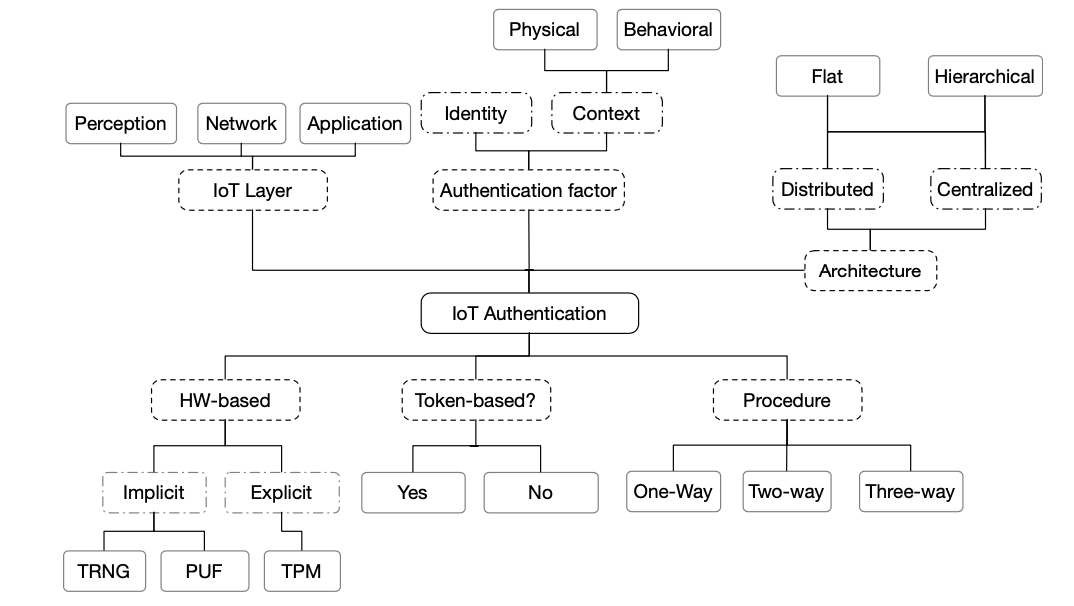
\includegraphics[scale=0.4]{resources/IoT_Auh_schems.png}


 Hier sind einige Klassifizierungen, die in \cite{khatoun2022cybersecurity} und [X3] erwähnt sind:

1. Authentifizierungsfaktor:
Identität: Informationen, die eine Partei der anderen zum Zwecke der Authentifizierung zur Verfügung stellt. Identitätsbasierte Authentifizierungsschemata können einen Hash-Algorithmus (oder eine Kombination davon), einen symmetrischen Verschlüsselungsalgorithmus oder einen asymmetrischen Verschlüsselungsalgorithmus verwenden.zum Beispiel Passwortbasierte Authentifizierung. 
Der Kontext kann physisch oder verhaltensbezogen sein. Ein Beispiel für einen physischen Kontext ist die biometrische Authentifizierung. 

2. Token-based:
Die Benutzer-/Geräteauthentifizierung basiert auf einem vom Server generierten Identitätstoken (Daten), wie z. B. das OAuth2-Protokoll oder Open ID . [X3]
Nicht-Token-basierte Authentifizierung: Die Verwendung der Anmeldeinformationen (Benutzername/Passwort) bei jedem Datenaustausch (z. B. TLS/DTLS [12,68,69]) [X3].

3. Authentifizierungsarchitektur
- Verteilt: Die Authentifizierung wird auf Knoten in der Nähe des Clients verteilt. 
Zentralisiert: Die Authentifizierung erfolgt über einen zentralen Server oder einen vertrauenswürdigen Dritten.

Hardware-basiert: Für den Authentifizierungsprozess sind möglicherweise physische Eigenschaften der Hardware oder der Hardware selbst erforderlich. - Implizit hardwarebasiert: nutzt physikalische Eigenschaften der Hardware, um die Authentifizierung zu verbessern, wie z. B. Physical Unclonable Function (PUF) oder True Random Number Generator (TRNG).
- Explizite Hardware-basiert: Einige Authentifizierungsmethoden basieren auf einem Trusted Platform Module (TPM), einem Chip (Hardware), der die für die Hardware-Authentifizierung verwendeten Schlüssel speichert und verarbeitet.

3. Authentifizierungsverfahren:
- Einweg-Authentifizierung (One-Way): Falls zwei Parteien miteinander kommunizieren möchten, wird nur eine Partei gegenüber der anderen authentifiziert und die andere Partei bleibt unauthentifiziert.


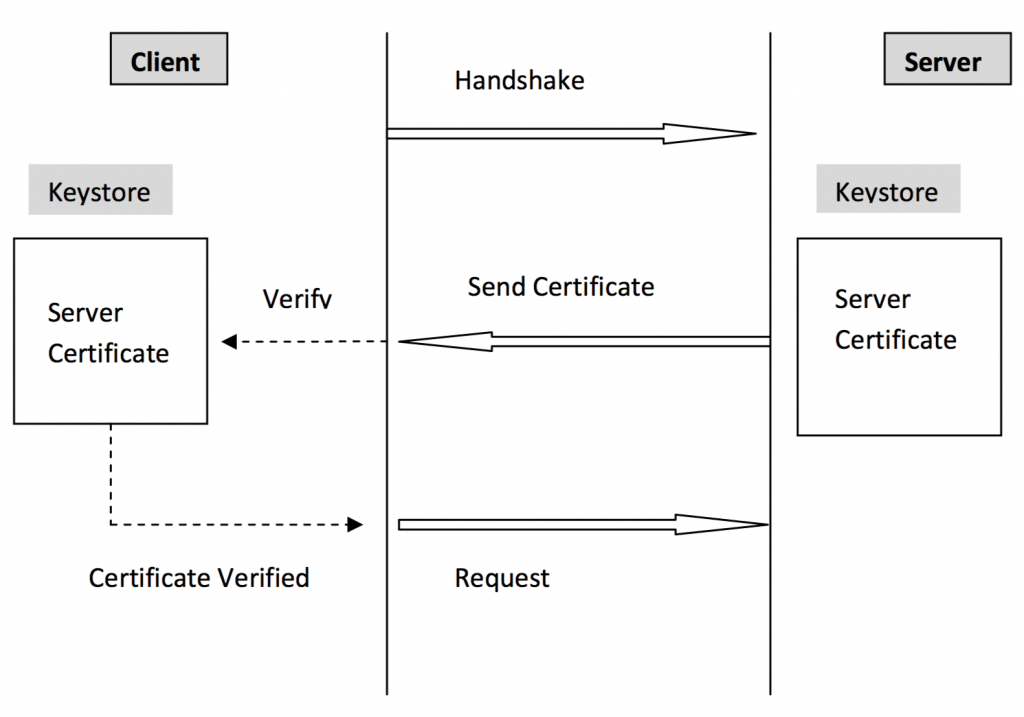
\includegraphics[scale=0.4]{resources/one-way-ssl.png}

 - Zwei-Wege-Authentifizierung (Mutual): Wird auch als gegenseitige Authentifizierung bezeichnet, wenn sich beide Parteien gegenseitig authentifizieren. Dies verhindert unbefugten Zugriff und Manipulation von Gerätezuständen. 
Es gibt verschiedene Methoden der gegenseitigen Authentifizierung: Verwendung eines öffentlichen Geheimnisses, eines öffentlichen Schlüssels oder eines Zeitstempels. 
1. Gegenseitige Authentifizierung unter Verwendung eines gemeinsamen Schlüssels:
 Partei A und Partei B teilen sich vorher sicher einen Schlüssel. Partei A sendet eine Nachricht an Partei B, die mit einer zufälligen Herausforderung antwortet. Teilnehmer A verschlüsselt die Verbindung mit dem gemeinsamen Schlüssel und sendet ihn zurück. Sie tauschen verschlüsselte Herausforderungen zur Authentifizierung aus.
 2. Gegenseitige Authentifizierung mittels Public-Key-Kryptographie:
Partei A und Partei B haben jeweils ein öffentlich-privates Schlüsselpaar. Wenn A mit B kommunizieren möchte, verschlüsselt A die Nachricht mit dem öffentlichen Schlüssel von B oder signiert sie mit seinem privaten Schlüssel. B entschlüsselt die Nachricht oder verifiziert die Signatur mit seinem privaten Schlüssel. 
Gegenseitige Authentifizierung mit Zeitstempeln:
Partei A sendet ihren aktuellen Benutzernamen und Zeitstempel, verschlüsselt mit einem gemeinsamen Schlüssel, an Partei B. B entschlüsselt den Zeitstempel, erhöht ihn, verschlüsselt den neuen Zeitstempel mit einem anderen gemeinsamen Schlüssel und sendet ihn zusammen mit dem Benutzernamen an Partei A zurück. Diese Methoden stellen sicher, dass beide Parteien sich gegenseitig authentifizieren, bevor sie Nachrichten austauschen, und verleihen dem Kommunikationsprozess eine zusätzliche Sicherheitsebene. 

-Drei-Wege-Authentifizierung(Three-Way): Hier authentifiziert die zentrale Autorität beide Parteien und hilft ihnen, sich gegenseitig zu authentifizieren.


\subsubsection{Mutual TLS}

Gegenseitiges TLS (mTLS), auch two-way TLS genannt, ist ein Sicherheitsmechanismus, der das herkömmliche TLS-Protokoll (Transport Layer Security) erweitert. Es bietet eine gegenseitige Authentifizierung zwischen Client und Server, indem beide Parteien ihre digitalen Zertifikate zur Überprüfung bereitstellen müssen.

Bei der gegenseitigen Authentifizierung authentifizieren sich Client und Server gegenseitig mit einem digitalen Zertifikat, z.B  X.509-Zertifikatstandard, bevor sie die Kommunikation herstellen. Das X.509-Zertifikat ist der anerkannte Standard zur Authentifizierung und Zugangskontrolle in Netzwerken. Sie bieten eine robuste Identitätsprüfung und sichere Kommunikation. Der weit verbreitete X.509-Zertifikatstandard umfasst einen öffentlichen Schlüssel, eine Identität, und kann von einer Zertifizierungsstelle (CA) signiert oder selbstsigniert werden.Der Prozess umfasst Root-CA-Zertifikate, Server-Zertifikate und Client-Zertifikate, die jeweils bestimmte Funktionen im Authentifizierungsprozess erfüllen (BUCH, X9).

Allerdings können IoT-Geräte aufgrund ihrer begrenzten Rechenleistung Schwierigkeiten mit komplexen kryptografischen Algorithmen haben.
Um dieses Problem zu lösen, wurden neuere IoT-Geräte mit mehr Standards und erhöhter Rechenleistung entwickelt, beispielsweise das Zertifikatformat IEEE 1609.2. Diese Geräte verwenden starke kryptografische Algorithmen, die speziell für IoT-Anwendungen optimiert sind. Dadurch wird die Authentifizierung und Sicherheit in IoT-Netzwerken verbessert, ohne die Ressourcen der Geräte übermäßig zu belasten.. \cite{khatoun2022cybersecurity}

\paragraph{Die gegenseitige TLS-Authentifizierung (mTLS) funktioniert folgendermaßen}
\

 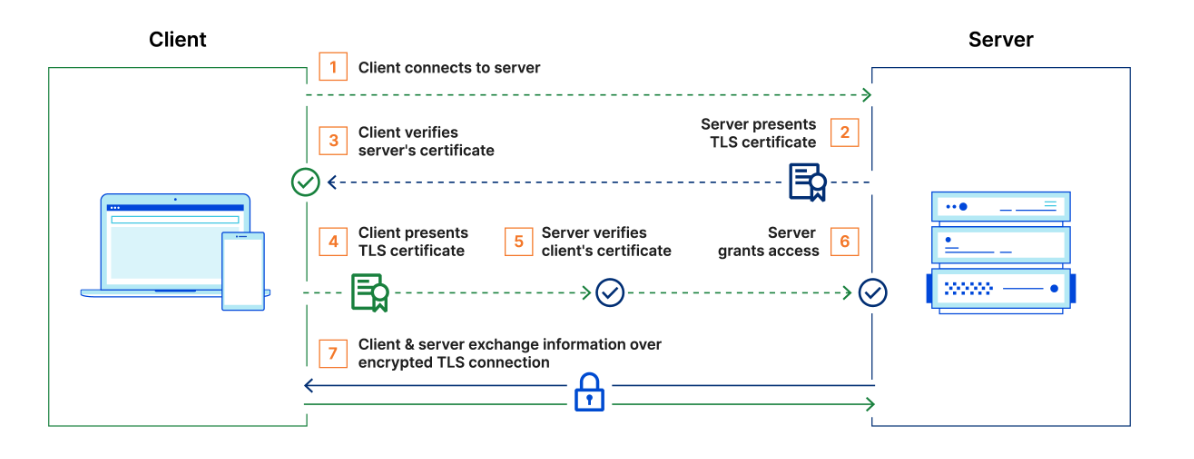
\includegraphics[scale=0.4]{resources/MUTUALTLS.png}
 
 der Client initiiert eine Verbindung zum Server. Der Server legt dem Client sein digitales Zertifikat vor, das vom Client mit Hilfe einer vertrauenswürdigen CA überprüft wird. Der Client legt dann sein eigenes Zertifikat zur gegenseitigen Authentifizierung vor, das der Server anhand einer vertrauenswürdigen CA verifiziert. Sobald beide Zertifikate erfolgreich verifiziert wurden, gewährt der Server dem Client Zugang und stellt eine sichere Verbindung für eine verschlüsselte und vertrauenswürdige Kommunikation her \cite{khatoun2022cybersecurity} und(X9).

\subsubsection{Lightweight CoAP-based Authentication }

CoAP ist eine schlanke Version von HTTP, die für Geräte mit eingeschränkten Ressourcen entwickelt wurde. In diesem Artikel [X6] wird eine vereinfachte Authentifizierungsmethode basierend auf CoAP vorgeschlagen. Dabei handelt es sich um einen einfachen Algorithmus, der eine zuverlässige Alternative zur komplexeren Data Transport Layer Security (DTLS) sein kann. Die Authentifizierung besteht aus vier Handshake-Nachrichten zwischen dem Client und dem Server unter Verwendung des 128-Bit Advanced Encryption Standard (AES). Jeder Client sendet vor Beginn der Authentifizierung einen 128-Bit-Pre-Shared-Key (Yi) an den Server. Jedem Gerät wird außerdem eine eindeutige Kennung zugewiesen, anhand derer der Server die Identität des Clients überprüft. Der Server verwaltet eine Pre-Shared-Key-Gruppe, die jeder Client-ID zugeordnet ist. Der Pre-Shared Key (Yi) ist nur dem Server und dem Client bekannt, mit dem er kommunizieren möchte. Die Authentifizierung beginnt mit der Sitzungsinitiierung. Wenn die Client-ID nicht überprüft wird, schlägt die Sitzung fehl.

Hier sind die Schritte des Authentifizierungsschemas:

\begin{enumerate}
    \item Session initiation:
    \item Server challenge:
    \item Client response and challenge:
    \item Server response:
\end{enumerate}

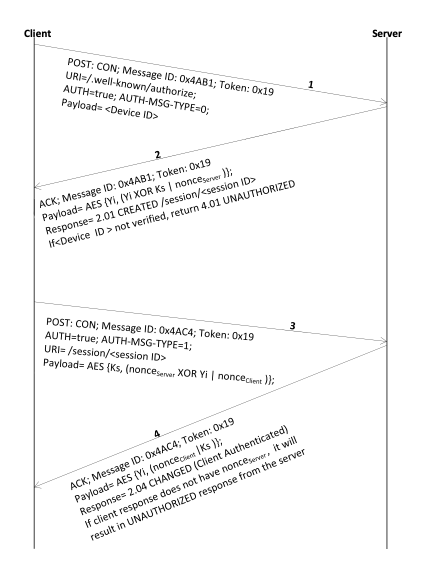
\includegraphics[scale=0.5]{resources/Lightweight CoAP-based Authentication.png}

\subsubsection{CoAP Payload Based Lightweight Authentication}

In [X7] wird eine neue Authentifizierungsmethode zwischen CoAP-Server und CoAP-Client vorgeschlagen. Diese Methode hat mehrere Vorteile: Sie erfordert keine zusätzlichen Protokolle, was die Komplexität und den Ressourcenbedarf reduziert. Es ermöglicht die gegenseitige Authentifizierung zwischen Geräten mit nur zwei Nachrichten. Bei der Authentifizierung wird nur eine kleine Datenmenge gesendet, etwa 300 Byte. Diese Methode ist schnell und effizient, da auf beiden Geräten nur ein Roundtrip und eine Verarbeitungszeit erforderlich ist.[x7]


Das funktioniert so: Wenn ein Client auf eine Ressource zugreifen möchte, muss er dem Server gegenüber seine Identität nachweisen. Nachdem der Server die Identität des Clients überprüft hat, erstellt er eine Sitzung für diesen Client und antwortet darauf. Nach Erhalt der Antwort authentifiziert der Client den Server. Wenn sich sowohl der Server als auch der Client gegenseitig authentifizieren, können sie mithilfe eines speziell für diese Sitzung generierten Sitzungsschlüssels Daten austauschen. Bei dieser Methode teilen sich Client und Server einen 128-Bit-AES-Schlüssel. Diese Schlüssel werden zum Zeitpunkt der Herstellung in das Gerät einprogrammiert, wobei davon ausgegangen wird, dass die Geräte vor physischen Angriffen geschützt sind. Darüber hinaus wird jedem Gerät bei der Herstellung eine eindeutige 64-Bit-ID zugewiesen.

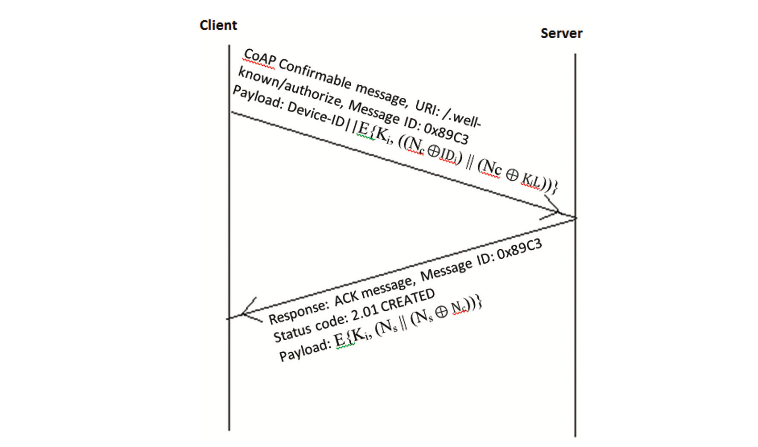
\includegraphics[scale=0.5]{resources/lightCo.png}


So funktioniert es im Detail:
Der Authentifizierungsprozess besteht aus drei Schritten: einmalige Gerätekonfiguration, Client-Authentifizierung und Server-Authentifizierung.

Die einmalige Gerätekonfiguration
Während der einmaligen Geräteeinrichtungsphase werden der eindeutige AES-Schlüssel und die eindeutige AES-ID in jedem Gerät fest codiert. Das Servergerät ist mit einer Tabelle konfiguriert, in der die Gerätekennung (IDi) und das gemeinsame Geheimnis (Ki) jedes Geräts gespeichert sind. Diese Tabelle wird verwendet, um das Gerät zu authentifizieren und den AES-Schlüssel während der ersten Servereinrichtung zu erhalten.

Die Client-Authentifizierung
Während des Client-Authentifizierungsschritts überprüft und authentifiziert der Server die Identität des Client-Geräts. Der Client generiert eine 64-Bit-Nonce (Nc) und XOR die Geräte-ID (IDi). Nonce wird außerdem mit den niedrigstwertigen 64 Bits des gemeinsamen Clientgeheimnisses (KiL) XOR-verknüpft.

C1 = E {Ki, ((Nc XOR IDi) || (Nc XOR KiL))}
M1p = IDi || C1

Der Client sendet dann eine CoAP-Nachricht (M1p) an den Server.Die payload der Nachricht enthält die Geräte-ID und einen verschlüsselten Teil (C1), der mit einem gemeinsamen Geheimnis generiert wird. Die Größe der Payload-Nachricht beträgt 192 Bit, einschließlich der unverschlüsselten Gerätekennung. Der Server empfängt diese Nachricht und liest daraus die Geräte-ID. Wenn die Geräte-ID in der Tabelle gefunden wird, wird der entsprechende Pre-Shared Key abgerufen. Anschließend entschlüsselt der Server den verschlüsselten Teil (C1) mit dem gemeinsamen geheimen Schlüssel (Ki), um den Klartext (P1) zu erhalten.
P1 = D{Ki, C1}


Die höchstwertigen 64 Bits von P1 werden mit der Gerätekennung IDi exklusiv-OR-verknüpft, was einen Wert Nc ergibt. Die niederwertigsten 64 Bits von P1 werden mit diesem Nc exklusiv-OR-verknüpft, was einen Wert R1 ergibt.


Der Server vergleicht den erhaltenen Wert R1 mit den niederwertigsten 64 Bits des geheimen Schlüssels, der mit der Geräteidentität IDi verknüpft ist. Wenn sie übereinstimmen, wird der Client authentifiziert und eine Sitzung zwischen Client und Server aufgebaut. Stimmen die Werte nicht überein, wird eine unautorisierte Nachricht an den Client gesendet, und es wird keine Sitzung aufgebaut.



Die Server-Authentifizierung


In der Server-Authentifizierungsphase erstellt der Server nach der Authentifizierung des Clients eine Antwortnachricht (M2p) mit dem Statuscode "2.01 created". Der Server generiert eine Nonce (Ns) und führt eine exklusive OR-Operation mit der Nonce des Clients (Nc) durch. 

M2p = E {Ki, (Ns || (Ns XOR Nc))}

Die daraus resultierende Nonce Ns wird dann mit der Verkettung der Nonce des Clients und der Nonce des Servers zu einem 128-Bit-Wert verkettet. Dieser Wert wird mit dem AES-Schlüssel verschlüsselt und als Payload der Antwortnachricht festgelegt.

Der Client empfängt die Antwortnachricht und entschlüsselt sie mit dem gemeinsamen geheimen Schlüssel (Ki).


P2 = D{Ki, M2p}

Die entschlüsselte Payload (M2p) wird dann verarbeitet, und die niedrigstwertigen 64 Bits des Klartextes (P2) werden mit den höchstwertigen 64 Bits von P2 exklusiv-OR-verknüpft, was zu einem Wert R2 führt.

Der Client vergleicht den Wert R2 mit seiner eigenen Nonce (Nc), um den Server zu authentifizieren. Wenn sie übereinstimmen, ist der Server authentifiziert, was bedeutet, dass nur der beabsichtigte Server die Nachricht des Clients entschlüsselt und die verschlüsselte Nonce zurückgeschickt haben kann.

Sobald die gegenseitige Authentifizierung zwischen Client und Server erreicht ist, wird ein Sitzungsschlüssel (Ks) durch Verkettung der Nonce des Clients (Nc) mit der Nonce des Servers (Ns) erzeugt. Dieser Sitzungsschlüssel wird zum Ver- und Entschlüsseln der während der authentifizierten Sitzung übertragenen Daten verwendet. Der während der Herstellungsphase gemeinsam genutzte AES-Schlüssel wird ausschließlich zu Authentifizierungszwecken verwendet, was die Sicherheit des Systems erhöht.




\subsection{Zugriffskontrolle und Berechtigungen}

By Zohreh:

Die Integration der physischen Welt und des Cybersystems im Internet der Dinge stellt große Herausforderungen an die Gestaltung von Sicherheitslösungen. Die Zugangskontrolle gilt als kritische Systemkomponente zum Schutz von Daten und Cyber-Infrastruktur. Aufgrund der neuen Eigenschaften von IoT-Systemen, wie z. B. viele traditionelle Sicherheitslösungen, einschließlich vorhandener Zugriffskontrollmechanismen, sind jedoch möglicherweise nicht direkt in der IoT-Umgebung anwendbar, z. B. Ressourcenbeschränkung, großer Umfang und Geräteheterogenität.\cite{8038503}\cite{ouaddah2017access}

\subsubsection{Zugriffskontrollmechanismen}

Ein vollständiges Zugangskontrollsystem besteht aus drei Funktionen: Authentifizierung, Autorisierung und Verantwortlichkeit. Der Zugriffskontrollmechanismus, der Hardware und Software umfasst, setzt Richtlinien durch und wertet Zugriffsanfragen aus. Die Konfiguration der Zugriffskontrollrichtlinien ist von entscheidender Bedeutung und sollte regelmäßig überprüft und verifiziert werden. Tools wie ACLs, Router, Verschlüsselung, Prüfprotokolle, IDS, Antivirensoftware, Firewalls, Smartcards und Warnungen sind Teil dieses Systems\cite{ouaddah2017access},\cite{vollbrecht2000rfc2904},\cite{boyle2007survey},\cite{hu2011anomaly},\cite{ledru2011validation}.
Es gibt viele verschiedene Zugriffskontrollmechanismen wie Role-Based Access Control (RBAC), Attribute-Based Access Control (ABAC) , Mandatory Access Control (MAC), Discretionary Access Control (DAC), Multi-Factor Authentication (MFA) und Single Sign-On (SSO) und Secure Shell (SSH), aber wir konzentrieren uns nur auf RBAC und ABAC\cite{ouaddah2017access}, \cite{coyne2013abac}, \cite{ameer2022hybrid}\cite{ali2019internet}\cite{dutta2020context}.

\subsubsection{RBAC und ABAC}

Obwohl ABAC und RBAC ähnlich sind, haben sie Vor- und Nachteile. Bei kluger Kombination kann die Kombination eine skalierbare, flexible, überprüfbare und verständliche Zugangskontrolle bieten. Durch die Kombination von Rollenzentrierung, dynamischen Rollenfunktionen und der feinkörnigen Autorisierung von ABAC demonstriert es die Praktikabilität des in ANSI/INCITS 494-2012 definierten Ansatzes und bietet eine Kombination der besten Funktionen von RBAC und ABAC für Unternehmen.
RBAC ist weit verbreitet und bietet Verwaltungs- und Sicherheitsvorteile. Es ist jedoch veraltet, teuer in der Implementierung und nicht in der Lage, Echtzeit-Umgebungszustände als Zugangskontrollparameter zu berücksichtigen. ABAC hingegen ist neuer, einfacher zu implementieren und kann Echtzeit-Umgebungszustände als Zugangskontrollparameter berücksichtigen.

Einerseits basiert die Zugriffskontrolle in RBAC auf vordefinierten Rollen und Berechtigungen, und Benutzerzugriffsentscheidungen hängen in erster Linie von den ihnen zugewiesenen Rollen ab. RBAC vereinfacht die Verwaltung, indem es die Zugriffskontrolle nach Rollen organisiert. Andererseits basiert die Zugriffskontrolle in ABAC auf verschiedenen Merkmalen von Benutzern, Objekten und der Umgebung, und Zugriffsentscheidungen berücksichtigen Attribute wie Benutzerrolle, Abteilung, Standort usw. ABAC bietet eine feinkörnige und kontextbezogene Steuerung von Genehmigung.

Sowohl RBAC als auch ABAC können verwendet werden, indem Rollen als Benutzerattribute betrachtet werden. RBAC vereinfacht die Administration und eignet sich für Organisationen mit komplexen Benutzerstrukturen. ABAC bietet Flexibilität, Granularität und feinkörnige Zugriffskontrolle. Darüber hinaus können Attribute zu RBAC hinzugefügt werden, um die erforderliche Flexibilität bei der Zugriffskontrolle zu erreichen.

RBAC ist einfacher zu implementieren, während ABAC eine Eigenschafts- und Richtlinienverwaltung erfordert. ABAC eignet sich besonders für dynamische Umgebungen und Attribute wie Tageszeit und Standort und ermöglicht eine effektive Richtliniendurchsetzung\cite{coyne2013abac}\cite{ameer2022hybrid}.

\subsubsection{HyBACAC}
Durch die vorteilhafte Kombination zweier Modelle, ABAC und R, als Hybridansatz steht eine umfassendere und wandelbarere Zutrittskontrolllösung zur Verfügung.
Ein von RBAC bereitgestelltes rollenzentriertes Framework vereinfacht die Administration und Zugriffsverwaltung, indem Berechtigungen an Rollen statt an einzelne Benutzer vergeben werden. Dies verbesserten die Skalierbarkeit und Ausdauer.
Andererseits kann ABAC eine feinkörnige Zugriffskontrolle unter Berücksichtigung der Attribute von Benutzern, Geräten und der Umgebung durchführen, was eine dynamische Entscheidungsfindung auf der Grundlage verschiedener Kontextfaktoren ermöglicht.
HyBACAC kann von der rollenbasierten Einfachheit von RBAC und der attributbasierten Flexibilität von ABAC profitieren. Diese Kombination erleichtert Administratoren das Definieren von Rollen und das Zuweisen geeigneter Berechtigungen, indem dynamische Attribute berücksichtigt werden, um den Zugriff weiter einzuschränken.
Es ermöglicht das Prinzip der geringsten Rechte und eine einfache Überprüfung der Benutzerberechtigungen.
Das Hybridmodell ist in der Lage, plötzliche Attributänderungen und Kontextinformationen durch dynamische Attribute und Umgebungsrollen zu erfassen. Dadurch wird sichergestellt, dass Entscheidungen zur Zugangskontrolle, an die sich ändernden Bedingungen in intelligenten IoT-Systemen angepasst werden können\cite{ameer2022hybrid}.


\newpage


\newpage
\section{Zusammenfassung}

By Zohreh:

Risikoanalyse ist die große Herausforderung für die Entwicklung von Smart-Home-Systemen.

Keywords: 
Smart Home Netzwerke, Architektur, Kommunikationsprotokolle, Bedrohungen, Risiken, Schutzmechanismen, Sicherheit, Verschlüsselung, Authentifizierung, Zugriffskontrolle, AES, BLOWFISH, RSA, Mutual TLS, Lightweight CoAP-based Authentication, CoAP Payload Based Lightweight Authentication, Zugriffskontrollmechanismen, IoT, Netzwerksicherheit, Datenschutz, Netzwerkarchitektur, Schwachstellen, Sicherheitslücken, Netzwerkprotokolle, Cybersecurity, Sichere Kommunikation, Risikomanagement.

\subsection{Ausblick auf zukünftige Entwicklungen und Forschungsbedarf}

Keywords:
Weiterentwicklung der Architektur, Erforschung neuer Kommunikationsprotokolle, Implementierung fortschrittlicher Sicherheitsmaßnahmen, Verschlüsselungstechnologien, Integration von KI- und ML-Lösungen, Entwicklung von Sicherheitsstandards, userfriendly, manageability.

\newpage

    \nocite{*}
    \bibliography{src/referencias}


\end{document}
